
\begin{frame}
  \frametitle{PySpice :  The Bridge between SPICE and Python}
  \textbf{How it is born ?}
  \begin{itemize}
  \item Come back to electronic learning
  \item Use the most maintained SPICE flavour : \textbf{NgSpice}
  \item But analysis tools are outdated : e.g. TCL Spice
  \item \textbf{I want Python !!!}
  \end{itemize}
  \vspace{1.5em}
  \centerline{\alert{$\Longrightarrow$ Plug NgSpice to Python}}
  \vspace{1.5em}
  \textbf{How to get it ?}
  \begin{itemize}
  \item Home \url{https://pyspice.fabrice-salvaire.fr}
  \item Code \url{https://github.com/FabriceSalvaire/PySpice}
  \item Available on PyPi
  \item Licensed under GPLv3
  \end{itemize}
\end{frame}

\begin{frame}
  \frametitle{PySpice: Workflow}
  \begin{center}
    \begin{tikzpicture}%
      [node distance=10mm,
      start chain=going right,
      >=stealth',
      punktchain/.style={
        rectangle,
        rounded corners,
        % fill=black!10,
        draw=black, very thick,
        text width=7em,
        minimum height=2em,
        text centered,
        on chain},
      line/.style={draw, thick, <-},
      element/.style={
        tape,
        top color=white,
        bottom color=blue!50!black!60!,
        minimum width=8em,
        draw=blue!40!black!90, very thick,
        text width=10em,
        minimum height=3.5em,
        text centered,
        on chain},
      every join/.style={->, thick,shorten >=1pt},
      decoration={brace},
      tuborg/.style={decorate},
      tubnode/.style={midway, right=2pt},
      ]
      \node[punktchain, join] {Python Netlist};
      \node[punktchain, join] {NgSpice};
      \node[punktchain, join] {Python Analysis};
    \end{tikzpicture}
  \end{center}
  \vspace{.5em}
  \begin{columns}[T]
    \begin{column}{.5\textwidth}
      \begin{enumerate}
      \item Define circuit in Python \\
        {
          \footnotesize
          \text{\colorR{C}\colorM{in} \colorB{1 2} \colorG{470n}}
          $\longrightarrow$
          \text{circuit.\colorR{C}(\colorM{'in'}, \colorB{1, 2}, \colorG{nano(470)})} \\[.5em]
        }
        or include netlist as is
      \item Define simulation parameters \\
      \item Generate netlist code \\
      \item Execute NgSpice \\
      \item Get output as Numpy array
      \item Analyse, plot \ldots
      \end{enumerate}
    \end{column}
    \begin{column}{.5\textwidth}
      Why Python Netlist ?
      \begin{itemize}
      \item More verbose, \textbf{But}
      \item Can use Python to configure netlist
        \href{https://pyspice.fabrice-salvaire.fr/examples/diode/voltage-multiplier.html}{example}
      \item keyword argument \\
        \texttt{resistance=kilo(100)}
      \item cf. Modelica \tiny{see later}
      \end{itemize}
    \end{column}
  \end{columns}
\end{frame}

\begin{frame}
  \frametitle{PySpice: I hate Netlist, I want schematic editor !!! }
  \centerline{\textbf{No Problem, Use \href{http://kicad-pcb.org}{KiCad}!}}
  \vspace{1em}
  \begin{columns}
    \begin{column}{.6\textwidth}
      \begin{itemize}
      \item Implement a minimal Netlist parser
      \item \alert{But a full parser would be difficult to implement} \\
        NgSpice syntax is very complex \\
        due to many extensions \\
        % And any grammar
      \item Tips: Use subcircuit to hide complexity
      \end{itemize}
    \end{column}
    \begin{column}{.4\textwidth}
      \begin{center}
        Leading Open Source \\
        Electronics Design Automation Suite \\[1em]
        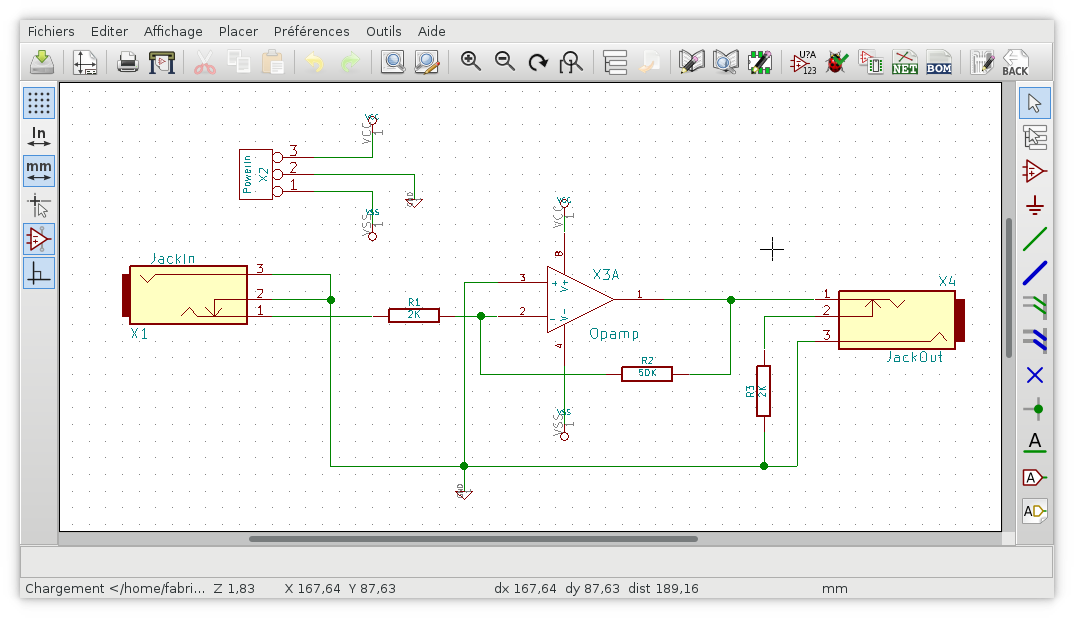
\includegraphics[width=1.\textwidth]{images/kicad.png}
      \end{center}
    \end{column}
  \end{columns}
  \vspace{1em}
  \centerline{\small \href{https://pyspice.fabrice-salvaire.fr/examples/spice-parser/kicad-example.html}{KiCad example}}
\end{frame}

\begin{frame}
  \frametitle{PySpice: NgSpice as a shared Library}
  \begin{itemize}
  \item NgSpice can be used as a shared library instead of an executable
  \item Not a big improvement, \textbf{But}
  \item We can use \textbf{NgSpice Shared API}
    \begin{itemize}
    \item To define external independent voltage/current sources (Input) % \\
      % API defines callback \\
      % \texttt{int (GetVSRCData)(double*, double, char*, int, void*)} \\
      % \texttt{int (GetISRCData)(double*, double, char*, int, void*)}
    \item To get the simulation output at each step (Output)
    \end{itemize}
    \alert{We can thus extend NgSpice easily with C or Python code}
    %
    % Add Picture ???  Python <-> NgSpice
    %
  \item API features also a step by step simulation mode
  \item PySpice as a \href{http://cffi.readthedocs.io/en/latest/}{CFFI} Binding
  \end{itemize}
  \vspace{1em}
  \centerline{\small \href{https://pyspice.fabrice-salvaire.fr/examples/ngspice-shared/voltage-divider.html}{NgSpice API example}}
\end{frame}

%%% Local Variables:
%%% mode: latex
%%% TeX-master: "master"
%%% End:
